% Definition der Klasse des Dokumentes
\documentclass[11pt, a4paper]{article}

\usepackage[T1]{fontenc}        % Sorgt u.a. dafür, dass Texte vernünftig markierbar werden auch bei Sonderzeichen
\usepackage{ae,aecompl} %bessere Schrift
\usepackage{gensymb}
\usepackage[ngerman]{babel}     % Deutsches Wörterbuch usw.
\usepackage{epstopdf}   % Wandelt .eps Dateien automatisch um
\usepackage{url}    % für URL mit \url{.....}
\usepackage[font=small,labelfont=bf]{caption}       % Optionen für Bild- und Codeunterschriften
\usepackage[hidelinks]{hyperref}                    % damit Links in der PDF anklickbar werden
\usepackage{booktabs}   % bessere Tabellen mit Abstand zur hline
\pagenumbering{arabic}
\usepackage[babel,german=guillemets]{csquotes} %deutsches Anführungszeichen
\usepackage{float} %bessere Positionierungsoptionen

% Standardpakete für deutsche Sprache
\usepackage[utf8]{inputenc}
\usepackage[ngerman]{babel}

% Volle Seite nutzen
\usepackage{fullpage} 
\headsep 1cm
\parindent 0cm

% einige Pakete für Mathematische Darstellung
\usepackage{amssymb, amstext, amsmath}
\usepackage{fancyhdr}

% ein Paket für die Zählung von Seiten
\usepackage{count1to}
\usepackage{lastpage} 

%Paket für Aufzählungsbuchstaben
\usepackage{enumitem}

\usepackage{nameref}



% HIER DIE NAMEN UND EMAIL ANPASSEN
\def \ATutantName{Moritz Breipohl}
\def \ATutantEmail{mbreipohl@techfak.uni-bielefeld.de}
\def \BTutantName{Markus Rothgänger}
\def \BTutantEmail{mrothgaenger@techfak.uni-bielefeld.de}
% HIER DIE VERSUCHSNUMMER ANPASSEN
\def \Versuchsnummer{Versuch 6}
% HIER DIE GRUPPENNUMMER ANPASSEN
\def \Gruppennummer{Gruppe 5}
% HIER DEN TUTORNAMEN ANPASSEN
\def \Tutorname{Lukas Schmidt, Robin Ewers}

% Kopfzeile und Fußzeile
\lhead{\Versuchsnummer}
\chead{\textbf{Digitalelektronisches Praktikum}}
\rhead{\today}
\lfoot{\Gruppennummer}
\rfoot{\thepage\ von \pageref{LastPage}}
\cfoot{}

% Wird zur Einbindung von Bildern benötigt
\usepackage{graphicx}
\graphicspath{{images/}}

% Physikalische Einheiten darstellen
\usepackage{siunitx}

% Einbinden des Literaturverzeichnisses
\usepackage[style=numeric-comp]{biblatex}
\bibliography{literatur.bib}

% Wird zum Einbinden von LaTeX Code benötigt
\usepackage{color}
\usepackage{showexpl}
\lstset
{
    language=[LaTeX]TeX,
    breaklines=true,
    basicstyle=\tt\scriptsize,
    keywordstyle=\color{blue},
    identifierstyle=\color{magenta},
}

\renewcommand{\footrulewidth}{0.4pt}
\pagestyle{fancy}

% Konfiguration des Deckblatts
\begin{titlepage}
\title{\textbf{Digitalelektronisches Praktikum\\ Versuch 6}}
\author{\ATutantName \\ \emph{\ATutantEmail} \and \BTutantName\\ \emph{\BTutantEmail}}
\date{\Gruppennummer \\[3ex] Tutor: \Tutorname \\[3ex] \today}
\end{titlepage}

\begin{document}
% Einfügen des Deckblatts
\clearpage
\maketitle
\thispagestyle{empty}
\newpage

%%%%%%%%%%%%%%%%%%%%%%%%%%%%%%%%%%%%%%%%%
%%% Ab hier Beginn des Laborberichts: %%%%%%%%%%%%%%%%%%%%%
\section*{Theorie/Allgemeines}
- Was ist ein FPGA?
- Schritte von graphischem Aufbau zu Bitsream / Schaltung
\section*{Versuchsaufbau}
Die allgemeine Benutzung der Software Vivado wird hier nicht erläutert.
\subsection*{Aufgabe}
Es wurden insgesamt sechs Aufgaben bearbeitet. Alle arbeiteten mit den Komponenten auf dem Board.
\begin{itemize}
	\item 1. In der ersten Aufgabe sollten sechs Segmente einer Sieben-Segment-Anzeige mit Hilfe von Vier Schaltern angesteuert werden.
	Dabei sollte der angezeigte Wert der Anzeige dem Binär kodierten Wert der Schalter entsprechen. Der Block zum Ansteuern der Sechs Segmente war vorgegeben. Die Funktionalität der Implementierung sollte (durch die Simulation mit der \textit{Testbench} und auf dem Board) verifiziert und die Aufgabe der \textit{Testbench} erklärt werden. Des weiteren sollte herausgearbeitet werden, welches Segment nicht angesteuert wird, sowie, welche Aufgabe das Ausgangssignal mit dem Code \textit{AN} besitzt.
	\item 2. Im zweiten Teil war die Schaltung aus der ersten Aufgabe zu erweitern, so dass auch das siebte Segment angesteuert wird. Dazu sollte eine aufgestellte Schaltlogik mithilfe des Karnaugh-Plans minimiert werden. Diese minimierte Schaltung wurde in das Block Design eingebaut. Auch dieses Block Design wurde durch die Simulation sowie am Board verifiziert.
	\item 3. Hier wurde das Erstellen eines \textit{IP-Core} (aus Zeitmangel) übersprungen. Es war herauszustellen, was bei dem Ansteuern aller vier Sieben-Segment-Anzeigen zu beachten ist. Diese Schaltung war zu skizzieren, zu implementieren und zu testen.
	\item 4. In der vierten Aufgabe sollten die mit den Schaltern eingestellten Werte erst bei einem Knopfdruck auf die Anzeige übernommen werden. Dazu waren alle möglichen Einbaustellen für Speicherelemente aufzuzählen und gegeneinander abzuwägen.
	Die Schaltung war zu implementieren und zu testen.
	\item 5. Im fünften Teil war das Zurücksetzen der Anzeige auf den Wert \textit{0000} bei Knopfdruck (eines weiteren Knopfes) zu implementieren. Es sollte erklärt werden, wieso sowohl der Knopf zum Zurücksetzen, als auch der Knopf zum Speichern zu drücken war, um die Anzeige zurückzusetzen.
	Eine Lösung dieses Problems war zu finden.
	\textit{\item 6. übersprungen}
	\item 7. Ein 16-Bit Zähler sollte erstellt werden, welcher bei einem Knopfdruck auf Null gesetzt werden konnte. Die Schaltung war zuerst mit zwei 8-Bit Addern zu skizzieren, dann zu realisieren und schließlich zu testen.
\end{itemize}
\subsection*{Aufbau und Erläuterung}
\subsubsection*{Verwendete Bauteile}
Basys 3 FPGA-Board, USB-Kabel, Computer mit Vivado Software.
\subsubsection*{Block Design Bauteile}
Hier eine Liste der Bauteile mit einer kurzen Erklärung der Funktionsweise
\begin{itemize}
	\item \textit{xlconstant:} Konstanter Wert dessen Bitweite eingestellt werden kann.
	\item \textit{xlslice:} Herausschneiden von bestimmten Bits des Eingangsbitstroms.
	\item \textit{xlconcat:} Hintereinanderfügen von zwei Bitströmen variabler Breite zu einem einzigen Bitstrom dessen Breite der Summe der Breiten der Eingangsbitströme entspricht.
\end{itemize}
\subsubsection*{Sechs-Segment-Anzeige}
\begin{figure}[htb]    
    \centering
    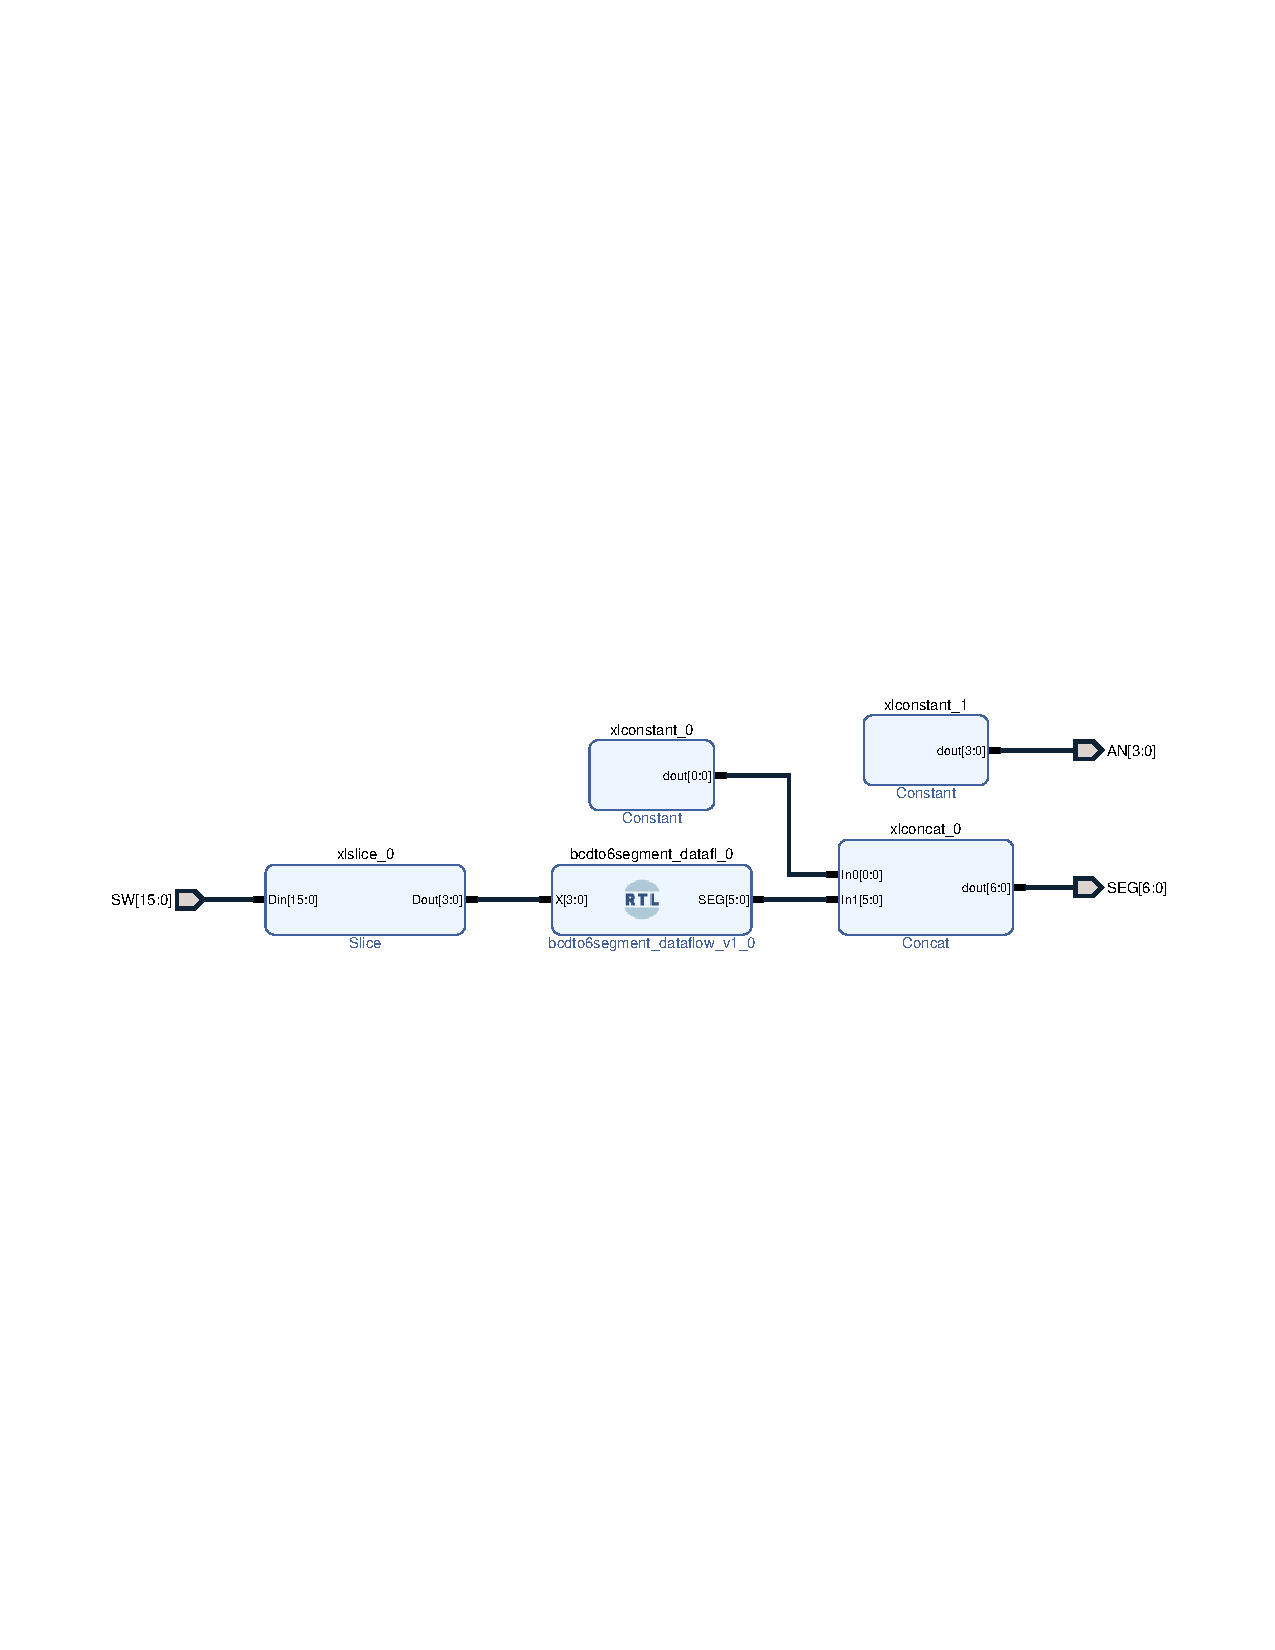
\includegraphics[width=\linewidth]{versuch1Data/seven_segment_display1.pdf}
    \caption{Block Design zum Ansteuern von Sechs der Sieben Segmente einer Anzeige}
    \label{aufbauSechsSegment}        
\end{figure}
Das Block Design zu dem ersten Aufbau war im wesentlichen Vorgegeben. Wie in \autoref{aufbauSechsSegment} zu sehen, wurde zuerst der Bitstrom aus dem Eingang der Schalter mit Hilfe des \textit{slice} Bausteins auf die unteren vier Bit verkleinert. Diese dienen dem aus den Aufgabendaten entnommenen Modul zum ansteuern der sechs Segmente als Eingang (in der Abbildung mit \textit{sw_to_6segment_dataf} bezeichnet). Der Ausgang des Moduls wurde mit einer ein Bit Konstante verknüpft und der sieben Bit breite Strom wurde an den Ausgang \textit{SEG} geleitet. Dieser steuert die Segmente direkt an.
Zusätzlich sollte eine vier Bit breite Konstante mit dem Wert 1 an den Ausgang \textit{AN} angelegt werden. Die Bedeutung dieses Wertes wird im folgenden Erläutert.
\subsubssubsection*{Test und Auswertung der Waveforms}
Bei einer Simulation mit der initialen Konfiguration läuft die Testbench auf einen Fehler. Dieser besagt, dass der Wert an der Anode falsch gesetzt ist. Ein Blick in das Handbuch des Boards klärt auf, dass die Anode den an dem Ausgang \textit{SEG} anliegenden Wert auf die Anzeigen weitergibt, für die das Bit an der Anode Null ist. Ein Binärcode von 1110 bedeutet also, dass die letzte Ziffer aktiv ist, die anderen nicht.
Ist der Wert der Konstante am Ausgang \textit{AN} also auf 14 (Wert des Binärcodes 1110) gesetzt, so läuft der Test ohne Fehler.
Hieraus wird deutlich, dass die Testbench die Funktionsweise und die Vorraussetzungen für eine spezifische Schaltung verifiziert, ähnlich zu einem Unit-Test.
\begin{figure}[htb]    
    \centering
    \includegraphics[width=\linewidth]{versuch1Data/waveform1.png}
    \caption{Block Design zum Ansteuern von Sechs der Sieben Segmente einer Anzeige}
    \label{aufbauSechsSegment}        
\end{figure}
\section*{Durchführung}. 
\section*{Messergebnisse}
\section*{Beobachtungen}
\section*{Auswertung}
\end{document}